%package list
\documentclass{article}
\usepackage[top=3cm, bottom=3cm, outer=3cm, inner=3cm]{geometry}
\usepackage{multicol}
\usepackage{graphicx}
\usepackage{url}
%\usepackage{cite}
\usepackage{hyperref}
\usepackage{array}
%\usepackage{multicol}
\newcolumntype{x}[1]{>{\centering\arraybackslash\hspace{0pt}}p{#1}}
\usepackage{natbib}
\usepackage{pdfpages}
\usepackage{multirow}
\usepackage[normalem]{ulem}
\useunder{\uline}{\ul}{}
\usepackage{svg}
\usepackage{xcolor}
\usepackage{listings}
\lstdefinestyle{ascii-tree}{
	literate={├}{|}1 {─}{--}1 {└}{+}1 
}
\lstset{basicstyle=\ttfamily,
	showstringspaces=false,
	commentstyle=\color{red},
	keywordstyle=\color{blue}
}
%\usepackage{booktabs}
\usepackage{caption}
\usepackage{subcaption}
\usepackage{float}
\usepackage{array}

\newcolumntype{M}[1]{>{\centering\arraybackslash}m{#1}}
\newcolumntype{N}{@{}m{0pt}@{}}


%%%%%%%%%%%%%%%%%%%%%%%%%%%%%%%%%%%%%%%%%%%%%%%%%%%%%%%%%%%%%%%%%%%%%%%%%%%%
%%%%%%%%%%%%%%%%%%%%%%%%%%%%%%%%%%%%%%%%%%%%%%%%%%%%%%%%%%%%%%%%%%%%%%%%%%%%
\newcommand{\itemEmail}{jchuraaca@unsa.edu.pe}
\newcommand{\itemStudent}{Julio Rubén Chura Acabana}
\newcommand{\itemCourse}{ F. de Programción 2}
\newcommand{\itemCourseCode}{20230472}
\newcommand{\itemSemester}{I}
\newcommand{\itemUniversity}{Universidad Nacional de San Agustín de Arequipa}
\newcommand{\itemFaculty}{Facultad de Ingeniería de Producción y Servicios}
\newcommand{\itemDepartment}{Departamento Académico de Ingeniería de Sistemas e Informática}
\newcommand{\itemSchool}{Escuela Profesional de Ingeniería de Sistemas}
\newcommand{\itemAcademic}{2023 - B}
\newcommand{\itemInput}{Del 18 Octubre 2023}
\newcommand{\itemOutput}{Al 23 Octubre 2023}
\newcommand{\itemPracticeNumber}{08}
\newcommand{\itemTheme}{HashMap}
%%%%%%%%%%%%%%%%%%%%%%%%%%%%%%%%%%%%%%%%%%%%%%%%%%%%%%%%%%%%%%%%%%%%%%%%%%%%
%%%%%%%%%%%%%%%%%%%%%%%%%%%%%%%%%%%%%%%%%%%%%%%%%%%%%%%%%%%%%%%%%%%%%%%%%%%%

\usepackage[english,spanish]{babel}
\usepackage[utf8]{inputenc}
\AtBeginDocument{\selectlanguage{spanish}}
\renewcommand{\figurename}{Figura}
\renewcommand{\refname}{Referencias}
\renewcommand{\tablename}{Tabla} %esto no funciona cuando se usa babel
\AtBeginDocument{%
	\renewcommand\tablename{Tabla}
}

\usepackage{fancyhdr}
\pagestyle{fancy}
\fancyhf{}
\setlength{\headheight}{30pt}
\renewcommand{\headrulewidth}{1pt}
\renewcommand{\footrulewidth}{1pt}
\fancyhead[L]{\raisebox{-0.2\height}{
\includegraphics[width=3cm]{img/logo_episunsa.png}}}
\fancyhead[C]{\fontsize{7}{7}\selectfont	\itemUniversity \\ \itemFaculty \\ \itemDepartment \\ \itemSchool \\ \textbf{\itemCourse}}
\fancyhead[R]{\raisebox{-0.2\height}{
\includegraphics[width=1.2cm]{img/logo_abet}}}
\fancyfoot[L]{Estudiante Julio Rubén Chura Acabana}
\fancyfoot[C]{\itemCourse}
\fancyfoot[R]{Página \thepage}

% para el codigo fuente
\usepackage{listings}
\usepackage{color, colortbl}
\definecolor{dkgreen}{rgb}{0,0.6,0}
\definecolor{gray}{rgb}{0.5,0.5,0.5}
\definecolor{mauve}{rgb}{0.58,0,0.82}
\definecolor{codebackground}{rgb}{0.95, 0.95, 0.92}
\definecolor{tablebackground}{rgb}{0.8, 0, 0}

\lstset{frame=tb,
	language=bash,
	aboveskip=3mm,
	belowskip=3mm,
	showstringspaces=false,
	columns=flexible,
	basicstyle={\small\ttfamily},
	numbers=none,
	numberstyle=\tiny\color{gray},
	keywordstyle=\color{blue},
	commentstyle=\color{dkgreen},
	stringstyle=\color{mauve},
	breaklines=true,
	breakatwhitespace=true,
	tabsize=3,
	backgroundcolor= \color{codebackground},
}

\begin{document}
	
	\vspace*{10px}
	
	\begin{center}	
		\fontsize{17}{17} \textbf{ Informe de Laboratorio \itemPracticeNumber}
	\end{center}
	\centerline{\textbf{\Large Tema: \itemTheme}}
	%\vspace*{0.5cm}	
	
	\begin{flushright}
		\begin{tabular}{|M{2.5cm}|N|}
			\hline 
			\rowcolor{tablebackground}
			\color{white} \textbf{Nota}  \\
			\hline 
			\\[30pt]
			\hline 			
		\end{tabular}
	\end{flushright}	
	
	\begin{table}[H]
		\begin{tabular}{|x{4.7cm}|x{4.8cm}|x{4.8cm}|}
			\hline 
			\rowcolor{tablebackground}
			\color{white} \textbf{Estudiante} & \color{white}\textbf{Escuela}  & \color{white}\textbf{Asignatura}   \\
			\hline 
			{\itemStudent \par \itemEmail} & \itemSchool & {\itemCourse \par Semestre: \itemSemester \par Código: \itemCourseCode}     \\
			\hline 			
		\end{tabular}
	\end{table}		
	
	\begin{table}[H]
		\begin{tabular}{|x{4.7cm}|x{4.8cm}|x{4.8cm}|}
			\hline 
			\rowcolor{tablebackground}
			\color{white}\textbf{Laboratorio} & \color{white}\textbf{Tema}  & \color{white}\textbf{Duración}   \\
			\hline 
			\itemPracticeNumber & \itemTheme & 04 horas   \\
			\hline 
		\end{tabular}
	\end{table}
	
	\begin{table}[H]
		\begin{tabular}{|x{4.7cm}|x{4.8cm}|x{4.8cm}|}
			\hline 
			\rowcolor{tablebackground}
			\color{white}\textbf{Semestre académico} & \color{white}\textbf{Fecha de inicio}  & \color{white}\textbf{Fecha de entrega}   \\
			\hline 
			\itemAcademic & \itemInput &  \itemOutput  \\
			\hline 
		\end{tabular}
	\end{table}
	
	\section{Tarea}
	\begin{itemize}		
		\item 
		Tendrá 2 Ejércitos. Inicializar el tablero con n soldados aleatorios entre 1 y 10 para cada 
		Ejército. Cada soldado tendrá un nombre autogenerado: Soldado0X1, Soldado1X1, etc., un 
		valor de puntos de vida autogenerado aleatoriamente [1..5], la fila y columna también 
		autogenerados aleatoriamente (no puede haber 2 soldados en el mismo cuadrado). Se debe 
		mostrar el tablero con todos los soldados creados (distinguir los de un ejército de los del otro 
		ejército). Además de los datos del Soldado con mayor vida de cada ejército, el promedio de 
		puntos de vida de todos los soldados creados por ejército, los datos de todos los soldados por 
		ejército en el orden que fueron creados y un ranking de poder de todos los soldados creados
		por ejército (del que tiene más nivel de vida al que tiene menos) usando 2 diferentes 
		Marco Aedo López 2
		algoritmos de ordenamiento. Finalmente, que muestre qué ejército ganará la batalla (indicar 
		la métrica usada para decidir al ganador de la batalla).
		\item Usted debe realizar varios commits y al término de la actividad deberá realizar un informe.
		
	\end{itemize}
	
	\section{Equipos, materiales y temas utilizados}
	\begin{itemize}
		\item Sistema Operativo Windows
		\item vim 9.0
		\item OpenJDK 64-Bits 20.0.2.
		\item Git 2.42.0.
		\item Cuenta en GitHub con el correo institucional.
		\item HashMap
	\end{itemize}
	
	\section{URL de Repositorio Github}
	\begin{itemize}
		\item URL del Repositorio GitHub para clonar o recuperar.
		\item \url{https://github.com/JulioChura/fp2-23b.git}
		\item URL para el laboratorio 01 en el Repositorio GitHub.
		\item \url{https://github.com/JulioChura/fp2-23b/tree/main/fase01/lab08}
	\end{itemize}
	
	\section{Actividades con el repositorio GitHub}
	
	\subsection{Creación y modificación de métodos}
	
	\begin{lstlisting}[language=bash,caption={Inicializando el espacio de trabajo}][H]
		mkdir lab08
		cd lab07
		Copy-Item "Soldier.java" -Destination "..\lab08"
		Copy-Item "VideoJuego4.java" -Destination "..\lab08\VideoJueg05.java"
		cd ..
		cd lab08
		vim VideoJuego5.java
	\end{lstlisting}
	
	\begin{lstlisting}[language=bash,caption={Commit: 04c6fccaf0efb49ff5850c22d6d70e304656daff }][H]
		git add Soldier.java
		git commit -m "Se copia la clase Soldier.java sin modificarla"
	\end{lstlisting}
	
	\begin{lstlisting}[language=bash,caption={Se modifica el método que genera un HashMap cuya llave es un String y el elemento es un Soldier }][H]
		vim VideoJuego5.java
	\end{lstlisting}
	\begin{figure}[H]
		\centering
		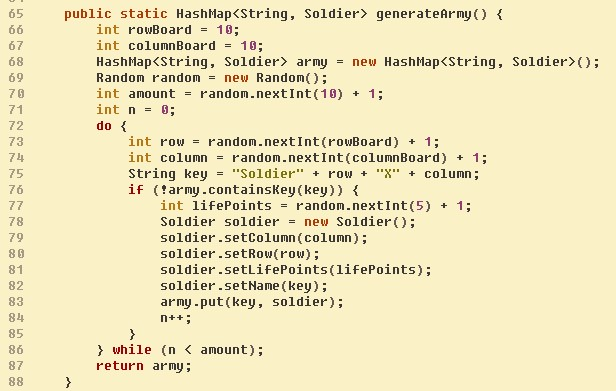
\includegraphics[width=1\textwidth,keepaspectratio]{img/generateArmy.jpg}
		%\includesvg{img/automata.svg}
		%\label{img:mot2}
		%\caption{Product backlog.}
	\end{figure}
	
	\begin{itemize}	
		\item El método generateArmy()  crea un HashMap cuya clave es de tipo String y es el nombre del Soldier. La razón de la elección de la clave es que las filas y columnas no se deben repetir por lo que guarda relación con la teoría que nos indica que las claves deben ser únicas.
		\item Para una mejor representación del Soldier en el tablero, se decide sumar uno a los números aleatorios que salgan de las row y column ya que el usuario no está acostumbrado a contar desde el 0.
	\end{itemize}
	
	
	\begin{lstlisting}[language=bash,caption={Commit: 0c0b73fb81d0a4ced7ff7998e9ed8dc40ac99f17}][H]
		git add VideoJuego5.java
		git commit -m "Se corrigen cosas del metodo generateArmy"			
		git push -u origin main
	\end{lstlisting}
	
	\begin{lstlisting}[language=bash,caption={Se modifica el método que genera un HashMap para el ejército B  }][H]
		vim VideoJuego5.java
	\end{lstlisting}
	
		\begin{figure}[H]
		\centering
		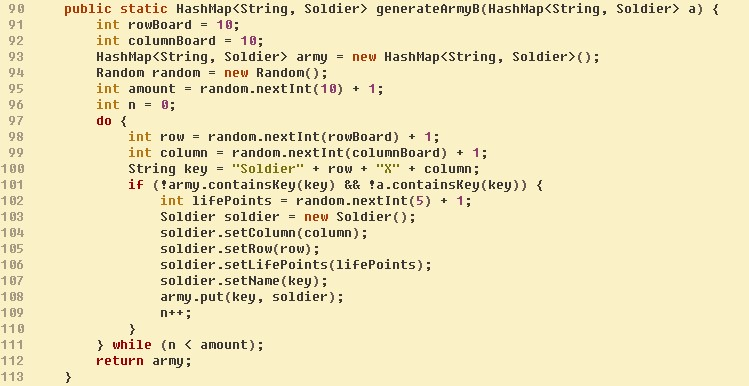
\includegraphics[width=1\textwidth,keepaspectratio]{img/generateArmyB.jpg}
		%\includesvg{img/automata.svg}
		%\label{img:mot2}
		%\caption{Product backlog.}
	\end{figure}
	
	\begin{itemize}	
		\item Este método recibe como parámetro un HashMap que es del ejercito A. Esto con el fin de garantizar que los elementos del ejército B se creén sin que hayan cruces con los del A.
		\item Se hace uso del método containsKey el cual nos retorna un boolean, siendo true que existe esa llave dentro del HashMap. Se hace uso en dos casos, uno es para garantizar que la llave que se ha creado sea única dentro del HashMap army y el otro para buscar coincidencias en el HashMap de a.
	\end{itemize}

	\begin{lstlisting}[language=bash,caption={Commit: c78e6ca75a2f9f69cc4559c9a8b598596b86b947}][H]
		git add VideoJuego5.java
		git commit -m "Se crea el metodo generateArmyB"			
		git push -u origin main
	\end{lstlisting}
		
	
	
	
	
	\begin{lstlisting}[language=bash,caption={Se modifica el método que imprime los datos de ambos ejércitos }][H]
		vim VideoJuego5.java
	\end{lstlisting}
	
	\begin{figure}[H]
		\centering
		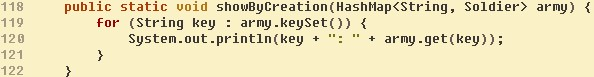
\includegraphics[width=1\textwidth,keepaspectratio]{img/showByCreation.jpg}
		%\includesvg{img/automata.svg}
		%\label{img:mot2}
		%\caption{Product backlog.}
	\end{figure}
	
	\begin{itemize}	
		\item Se opta por modificar el método ya realizado de la actividad de laboratorio anterior por lo que ya se podrá imprimir HashMap.
	\end{itemize}
	
	
	\begin{lstlisting}[language=bash,caption={ Probando los métodos}][H]
		javac VideoJuego5.java
		java VideoJuego5
		Desea jugar una ronda?(si/no)
		si
		oooooooooooooooo  FASE 1 DE LA CONTIENDA  oooooooooooooooo
		Mostrando estadisticas de cada ejercito
		
		Mostrando soldados por orden de creacion
		DATOS DEL DEL EJERCITO A
		Soldier9X9: Soldier [name=Soldier9X9, lifePoints=3, row=10, column=10]
		Soldier5X4: Soldier [name=Soldier5X4, lifePoints=1, row=6, column=5]
		Soldier4X5: Soldier [name=Soldier4X5, lifePoints=2, row=5, column=6]
		Soldier10X9: Soldier [name=Soldier10X9, lifePoints=3, row=11, column=10]
		Soldier2X4: Soldier [name=Soldier2X4, lifePoints=4, row=3, column=5]
		Soldier2X5: Soldier [name=Soldier2X5, lifePoints=1, row=3, column=6]
		Soldier8X4: Soldier [name=Soldier8X4, lifePoints=1, row=9, column=5]
		Soldier3X9: Soldier [name=Soldier3X9, lifePoints=3, row=4, column=10]
		DATOS DEL EJRCITO B
		Soldier5X3: Soldier [name=Soldier5X3, lifePoints=5, row=6, column=4]
		Soldier2X7: Soldier [name=Soldier2X7, lifePoints=5, row=3, column=8]
		Soldier2X8: Soldier [name=Soldier2X8, lifePoints=2, row=3, column=9]
		Soldier2X10: Soldier [name=Soldier2X10, lifePoints=2, row=3, column=11]
		Desea jugar una ronda?(si/no)
		no
		
	\end{lstlisting}
	
	\begin{itemize}	
		\item No damos cuenta que la llave de cada Soldier no coincide con la fila y columna, este problema se debe a los accesores de row y column ya que a cada uno se les suma 1.
	\end{itemize}
	
	
	\begin{lstlisting}[language=bash,caption={Commit: 8d7511cfd2f009ae04e1691cf9f2f85b3c80b0f7}][H]
		git add VideoJuego5.java
		git commit -m "Se modifica el metodo showByCreation"			
		git push -u origin main
	\end{lstlisting}
	
	
	
	
	
	

	
	
	
	
	
	\begin{lstlisting}[language=bash,caption={Se modifica la clase Soldier}][H]
		vim Soldier.java
	\end{lstlisting}
	
	\begin{figure}[H]
		\centering
		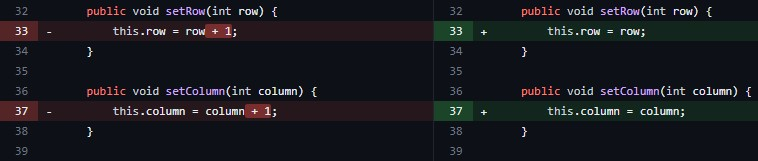
\includegraphics[width=1\textwidth,keepaspectratio]{img/classSoldier.jpg}
		%\includesvg{img/automata.svg}
		%\label{img:mot2}
		%\caption{Product backlog.}
	\end{figure}
	
	\begin{itemize}	
		\item Se le borra +1 tanto a los métodos setColumn y setRow ya que de no hacerlo se presentaría el problema de desbordamiento.
	\end{itemize}
	
	\begin{lstlisting}[language=bash,caption={Compilando y probando}][H]
		javac VideoJuego5.java
		java VideoJuego5
		Desea jugar una ronda?(si/no)
		si
		oooooooooooooooo  FASE 1 DE LA CONTIENDA  oooooooooooooooo
		Mostrando estadisticas de cada ejercito
		
		Mostrando soldados por orden de creacion
		DATOS DEL DEL EJERCITO A
		Soldier3X2: Soldier [name=Soldier3X2, lifePoints=4, row=3, column=2]
		Soldier6X1: Soldier [name=Soldier6X1, lifePoints=2, row=6, column=1]
		Soldier10X7: Soldier [name=Soldier10X7, lifePoints=3, row=10, column=7]
		Soldier8X8: Soldier [name=Soldier8X8, lifePoints=1, row=8, column=8]
		DATOS DEL EJRCITO B
		Soldier7X1: Soldier [name=Soldier7X1, lifePoints=5, row=7, column=1]
		Soldier10X9: Soldier [name=Soldier10X9, lifePoints=3, row=10, column=9]
		Soldier5X1: Soldier [name=Soldier5X1, lifePoints=1, row=5, column=1]
		Soldier10X5: Soldier [name=Soldier10X5, lifePoints=5, row=10, column=5]
		Desea jugar una ronda?(si/no)
		no
	\end{lstlisting}
	
	\begin{itemize}	
		\item Ahora si coinciden las llaves y la posición de cada Soldier.
	\end{itemize}
	
		
	\begin{lstlisting}[language=bash,caption={Commit: a13e2f09357ac8e78d9aa0a0c1aa9e654a0a09df}][H]
		git add VideoJuego5.java
		git commit -m "Se borra mas uno en los setColumn y setRow"			
		git push -u origin main
	\end{lstlisting}
	
	
	
	\begin{lstlisting}[language=bash,caption={Se modifica el metodo LongerLife}][H]
		vim VideoJuego5.java
	\end{lstlisting}
	
	\begin{figure}[H]
		\centering
		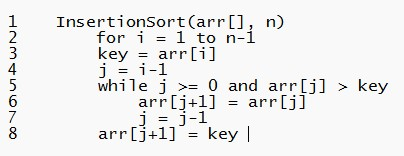
\includegraphics[width=1\textwidth,keepaspectratio]{img/insertion.jpg}
		%\includesvg{img/automata.svg}
		%\label{img:mot2}
		%\caption{Product backlog.}
	\end{figure}
	
		\begin{itemize}	
		\item Este el pseudocódigo del ordenamiento por inserción a un Arreglo Estándar.
	\end{itemize}
	
	
	\begin{figure}[H]
		\centering
		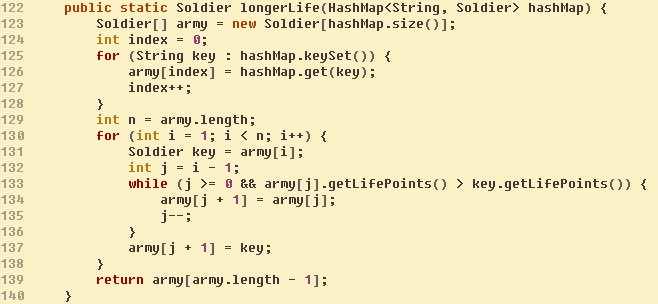
\includegraphics[width=1\textwidth,keepaspectratio]{img/longerLife.jpg}
		%\includesvg{img/automata.svg}
		%\label{img:mot2}
		%\caption{Product backlog.}
	\end{figure}
	
	\begin{itemize}	
		\item Recordemos que un Hash Map no se puede ordenar de manera directa, por lo que se opta de pasar los elementos del Hash Map a un arreglo Estándar de tipo Soldier. No nos preocupamos por las llaves ya que prácticamente vendría a ser lo mismo que los nombres de cada Soldier. 
		\item Una vez trasladados los elementos al arreglo Estándar, se hace uso del algoritmo de ordenamiento por inserción. Finalmente se retorna un Soldier de la última posición del arreglo porque está ordenado de manera ascendente.
	\end{itemize}
	
	\begin{lstlisting}[language=bash,caption={Compilando y probando}][H]
		javac VideoJuego5.java
		java VideoJuego5
		Desea jugar una ronda?(si/no)
		si
		oooooooooooooooo  FASE 1 DE LA CONTIENDA  oooooooooooooooo
		Mostrando estadisticas de cada ejercito
		
		Mostrando soldados por orden de creacion
		DATOS DEL DEL EJERCITO A
		Soldier4X4: Soldier [name=Soldier4X4, lifePoints=2, row=4, column=4]
		Soldier5X2: Soldier [name=Soldier5X2, lifePoints=2, row=5, column=2]
		Soldier9X3: Soldier [name=Soldier9X3, lifePoints=1, row=9, column=3]
		Soldier4X8: Soldier [name=Soldier4X8, lifePoints=2, row=4, column=8]
		Soldier4X7: Soldier [name=Soldier4X7, lifePoints=3, row=4, column=7]
		Soldier9X2: Soldier [name=Soldier9X2, lifePoints=2, row=9, column=2]
		Soldier6X8: Soldier [name=Soldier6X8, lifePoints=5, row=6, column=8]
		Mayor vida en A: Soldier [name=Soldier6X8, lifePoints=5, row=6, column=8]
		DATOS DEL EJRCITO B
		Soldier4X9: Soldier [name=Soldier4X9, lifePoints=4, row=4, column=9]
		Soldier3X7: Soldier [name=Soldier3X7, lifePoints=3, row=3, column=7]
		Soldier9X7: Soldier [name=Soldier9X7, lifePoints=5, row=9, column=7]
		Mayor vida en B: Soldier [name=Soldier9X7, lifePoints=5, row=9, column=7]
		Desea jugar una ronda?(si/no)
		no
	\end{lstlisting}

	\begin{lstlisting}[language=bash,caption={Commit: 34a06097f486f0e96e4785f39e9311c655287aa7}][H]
		git add VideoJuego5.java
		git commit -m "Se adapata el metodo longerLife para un HashMap"			
		git push -u origin main
	\end{lstlisting}
	
	

	
	
	\begin{lstlisting}[language=bash,caption={Se modifica el método retorna la suma de la cantidad de puntos del ejército}][H]
		vim VideoJuego5.java
	\end{lstlisting}
	
	\begin{figure}[H]
		\centering
		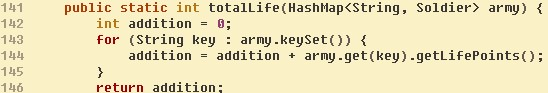
\includegraphics[width=1\textwidth,keepaspectratio]{img/totalLife.jpg}
		%\includesvg{img/automata.svg}
		%\label{img:mot2}
		%\caption{Product backlog.}
	\end{figure}
	
		
	\begin{itemize}	
		\item Se hace uso del método keySet para poder acceder a todas llaves y valores. Luego de sacar el valor se le saca sus puntos de vida con el método getLifePoints y se procede a ir sumando los puntos de vida.
	\end{itemize}
	
	
	\begin{lstlisting}[language=bash,caption={Compilando y probando }][H]
		javac VideoJuego5.java
		java VideoJuego5
		Desea jugar una ronda?(si/no)
		si
		oooooooooooooooo  FASE 1 DE LA CONTIENDA  oooooooooooooooo
		Mostrando estadisticas de cada ejercito
		
		Mostrando soldados por orden de creacion
		DATOS DEL DEL EJERCITO A
		Soldier1X10: Soldier [name=Soldier1X10, lifePoints=2, row=1, column=10]
		Soldier5X2: Soldier [name=Soldier5X2, lifePoints=2, row=5, column=2]
		Soldier7X5: Soldier [name=Soldier7X5, lifePoints=1, row=7, column=5]
		Soldier8X4: Soldier [name=Soldier8X4, lifePoints=1, row=8, column=4]
		Soldier5X8: Soldier [name=Soldier5X8, lifePoints=4, row=5, column=8]
		Soldier8X8: Soldier [name=Soldier8X8, lifePoints=3, row=8, column=8]
		Soldier8X9: Soldier [name=Soldier8X9, lifePoints=1, row=8, column=9]
		Soldier3X10: Soldier [name=Soldier3X10, lifePoints=5, row=3, column=10]
		Mayor vida en A: Soldier [name=Soldier3X10, lifePoints=5, row=3, column=10]
		El total de vida del ejercito A es: 19
		DATOS DEL EJRCITO B
		Soldier9X9: Soldier [name=Soldier9X9, lifePoints=5, row=9, column=9]
		Soldier2X1: Soldier [name=Soldier2X1, lifePoints=2, row=2, column=1]
		Soldier3X5: Soldier [name=Soldier3X5, lifePoints=2, row=3, column=5]
		Soldier4X2: Soldier [name=Soldier4X2, lifePoints=5, row=4, column=2]
		Soldier9X8: Soldier [name=Soldier9X8, lifePoints=5, row=9, column=8]
		Mayor vida en B: Soldier [name=Soldier9X8, lifePoints=5, row=9, column=8]
		El total de vida del ejercito B es: 19
		Desea jugar una ronda?(si/no)
		no
	\end{lstlisting}
	
	\begin{lstlisting}[language=bash,caption={Commit: 8c68956fc2e3f75c1fd1b3c7bd5919f5b50c9416}][H]
		git add VideoJuego5.java
		git commit -m "Se culmina el metodo totalLife"			
		git push -u origin main
	\end{lstlisting}
	
	
	\begin{lstlisting}[language=bash,caption={Se calcula el promedio de vida de cada ejército}][H]
		vim VideoJuego5.java
	\end{lstlisting}
	
	\begin{figure}[H]
		\centering
		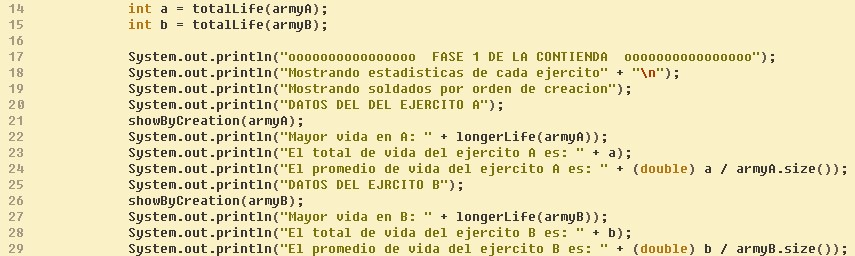
\includegraphics[width=1\textwidth,keepaspectratio]{img/average.jpg}
		%\includesvg{img/automata.svg}
		%\label{img:mot2}
		%\caption{Product backlog.}
	\end{figure}
	
	
	\begin{itemize}	
		\item En la línea 14 y 15 de la imagen, se puede observar que los puntos de vida total de cada ejército son recibidos por dos variables.
		\item En la línea 24 se observa que se imprime un mensaje que nos indica el promedio de vida del ejército A. Del mismo modo, en la linea 29 se hace lo mismo, pero para el ejército B.
	\end{itemize}
	
	\begin{lstlisting}[language=bash,caption={Commit: ac8683975133d422bba4e6f0c13a5c378a38e50d}][H]
		git add VideoJuego5.java
		git commit -m "Se calcula el promedio de vida de cada ejercito"			
		git push -u origin main
	\end{lstlisting}	
	
	
	
	\begin{lstlisting}[language=bash,caption={Se modifica el método que imprime el ranking de poder}][H]
		vim VideoJuego5.java
	\end{lstlisting}
	
	\begin{figure}[H]
		\centering
		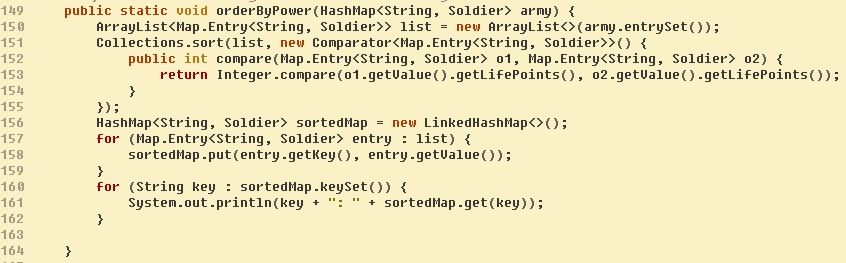
\includegraphics[width=1\textwidth,keepaspectratio]{img/orderByPower.jpg}
		%\includesvg{img/automata.svg}
		%\label{img:mot2}
		%\caption{Product backlog.}
	\end{figure}
	
	
	\begin{itemize}	
		\item Como ya se mencionó, un HashMap no puede ser ordenado de forma directa. Más antes se propuso un enfoque de trasladar los datos a un arreglo Estándar y luego aplicar el algoritmo de inserción, no obstante, en este método se propone usar un método de los List el cual es Collections.sort, sin embargo, no puede ser aplicado a un Map, por lo que primero se opta por pasar los datos a un ArrayList y luego modificar el Comparator para personalizar las comparaciones que determinarán el orden. Luego movemos esos resultados a un LinkedHashMap el cual mantiene el orden. Finalmente se mostrarán los elementos ya ordenados.
	\end{itemize}
	
	
	\begin{lstlisting}[language=bash,caption={Compilando y probando }][H]
	javac VideoJuego5.java
	java VideoJuego5
	Desea jugar una ronda?(si/no)
	si
	oooooooooooooooo  FASE 1 DE LA CONTIENDA  oooooooooooooooo
	Mostrando estadisticas de cada ejercito
	
	Mostrando soldados por orden de creacion
	DATOS DEL DEL EJERCITO A
	Soldier5X3: Soldier [name=Soldier5X3, lifePoints=1, row=5, column=3]
	Soldier6X3: Soldier [name=Soldier6X3, lifePoints=3, row=6, column=3]
	Soldier10X8: Soldier [name=Soldier10X8, lifePoints=4, row=10, column=8]
	Soldier2X4: Soldier [name=Soldier2X4, lifePoints=1, row=2, column=4]
	Soldier8X2: Soldier [name=Soldier8X2, lifePoints=5, row=8, column=2]
	Mayor vida en A: Soldier [name=Soldier8X2, lifePoints=5, row=8, column=2]
	El total de vida del ejercito A es: 14
	El promedio de vida del ejercito A es: 2.8
	Mostrando soldados por ranking de poder de A
	Soldier5X3: Soldier [name=Soldier5X3, lifePoints=1, row=5, column=3]
	Soldier2X4: Soldier [name=Soldier2X4, lifePoints=1, row=2, column=4]
	Soldier6X3: Soldier [name=Soldier6X3, lifePoints=3, row=6, column=3]
	Soldier10X8: Soldier [name=Soldier10X8, lifePoints=4, row=10, column=8]
	Soldier8X2: Soldier [name=Soldier8X2, lifePoints=5, row=8, column=2]
	DATOS DEL EJRCITO B
	Soldier2X5: Soldier [name=Soldier2X5, lifePoints=4, row=2, column=5]
	Soldier5X8: Soldier [name=Soldier5X8, lifePoints=1, row=5, column=8]
	Soldier7X3: Soldier [name=Soldier7X3, lifePoints=1, row=7, column=3]
	Soldier5X9: Soldier [name=Soldier5X9, lifePoints=4, row=5, column=9]
	Mayor vida en B: Soldier [name=Soldier5X9, lifePoints=4, row=5, column=9]
	El total de vida del ejercito B es: 10
	El promedio de vida del ejercito B es: 2.5
	Mostrando soldados por ranking de poder de B
	Soldier5X8: Soldier [name=Soldier5X8, lifePoints=1, row=5, column=8]
	Soldier7X3: Soldier [name=Soldier7X3, lifePoints=1, row=7, column=3]
	Soldier2X5: Soldier [name=Soldier2X5, lifePoints=4, row=2, column=5]
	Soldier5X9: Soldier [name=Soldier5X9, lifePoints=4, row=5, column=9]
	Desea jugar una ronda?(si/no)
	no
	\end{lstlisting}
	
	
	\begin{lstlisting}[language=bash,caption={Commit: d3af64e3678b36984d744ac19d598ea08e012bee}][H]
		git add VideoJuego5.java
		git commit -m "Metodo orderByPower culminado"			
		git push -u origin main
	\end{lstlisting}	
	
	
	
	\begin{lstlisting}[language=bash,caption={Se implementa el método que hace una búsqueda binaria del nombre solicitado}][H]
		vim VideoJuego5.java
	\end{lstlisting}
	
	\begin{figure}[H]
		\centering
		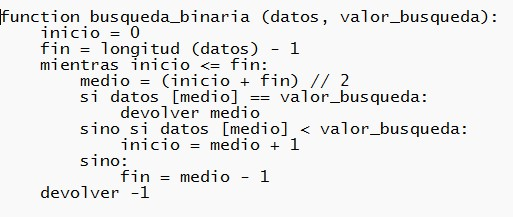
\includegraphics[width=1\textwidth,keepaspectratio]{img/binary.jpg}
		%\includesvg{img/automata.svg}
		%\label{img:mot2}
		%\caption{Product backlog.}
	\end{figure}
	
	
	\begin{itemize}	
		\item Este es el pseudocódigo de búsqueda binaria.
	\end{itemize}
	
	\begin{figure}[H]
		\centering
		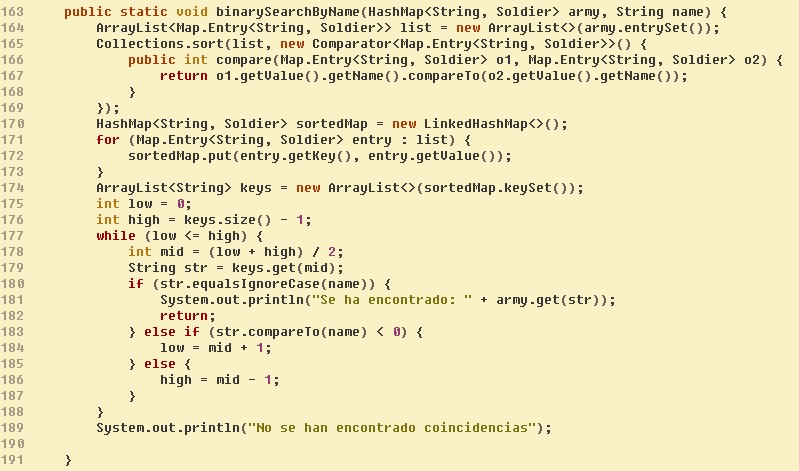
\includegraphics[width=1\textwidth,keepaspectratio]{img/binarySearchByName.jpg}
		%\includesvg{img/automata.svg}
		%\label{img:mot2}
		%\caption{Product backlog.}
	\end{figure}
	
	
	\begin{itemize}	
		\item Primero, se convierten los elementos del HashMap en una lista de Map.Entry, que contiene tanto las claves (nombres) como los valores (objetos Soldier). Luego se ordena esta lista de Map.Entry en función del nombre de los Soldier utilizando Collections.sort.
		Posteriormente se crea un nuevo LinkedHashMap llamado sortedMap para mantener los elementos ordenados, y se copian los elementos ordenados en él. Luego se crea un ArrayList llamado keys que contiene las llaves en el orden deseado, que es el orden alfabético de los nombres de los soldados. Luego se realiza la búsqueda binaria en el ArrayList de llaves (keys). 
	\end{itemize}
	
	
	
	
	\begin{lstlisting}[language=bash,caption={Compilando y probando }][H]
		javac VideoJuego5.java
		java VideoJuego5
		Desea jugar una ronda?(si/no)
		si
		oooooooooooooooo  FASE 1 DE LA CONTIENDA  oooooooooooooooo
		Mostrando estadisticas de cada ejercito
		
		Mostrando soldados por orden de creacion
		DATOS DEL DEL EJERCITO A
		Soldier9X4: Soldier [name=Soldier9X4, lifePoints=1, row=9, column=4]
		Soldier5X5: Soldier [name=Soldier5X5, lifePoints=1, row=5, column=5]
		Mayor vida en A: Soldier [name=Soldier5X5, lifePoints=1, row=5, column=5]
		El total de vida del ejercito A es: 2
		El promedio de vida del ejercito A es: 1.0
		Mostrando soldados por ranking de poder de A
		Soldier9X4: Soldier [name=Soldier9X4, lifePoints=1, row=9, column=4]
		Soldier5X5: Soldier [name=Soldier5X5, lifePoints=1, row=5, column=5]
		Ingrese el nombre del Soldier que desea buscar
		soldier9x4
		Se ha encontrado: Soldier [name=Soldier9X4, lifePoints=1, row=9, column=4]
		DATOS DEL EJRCITO B
		Soldier4X8: Soldier [name=Soldier4X8, lifePoints=1, row=4, column=8]
		Soldier9X3: Soldier [name=Soldier9X3, lifePoints=2, row=9, column=3]
		Soldier10X1: Soldier [name=Soldier10X1, lifePoints=2, row=10, column=1]
		Mayor vida en B: Soldier [name=Soldier10X1, lifePoints=2, row=10, column=1]
		El total de vida del ejercito B es: 5
		El promedio de vida del ejercito B es: 1.6666666666666667
		Mostrando soldados por ranking de poder de B
		Soldier4X8: Soldier [name=Soldier4X8, lifePoints=1, row=4, column=8]
		Soldier9X3: Soldier [name=Soldier9X3, lifePoints=2, row=9, column=3]
		Soldier10X1: Soldier [name=Soldier10X1, lifePoints=2, row=10, column=1]
		Ingrese el nombre del Soldier que desea buscar
		soldier9x3
		Se ha encontrado: Soldier [name=Soldier9X3, lifePoints=2, row=9, column=3]
		Desea jugar una ronda?(si/no)
		no
	\end{lstlisting}
	
	
	
	\begin{lstlisting}[language=bash,caption={Commit: 556b06b12e835c82e309c4ad3dcde5ced22e2b94}][H]
		git add VideoJuego5.java
		git commit -m "Metodo binarySearchByName culminado"			
		git push -u origin main
	\end{lstlisting}
	

	
	\begin{lstlisting}[language=bash,caption={Se implementa el método que hace la búsqueda secuencial de un Soldier por su nombre}][H]
		vim VideoJuego5.java
	\end{lstlisting}
	
	\begin{figure}[H]
		\centering
		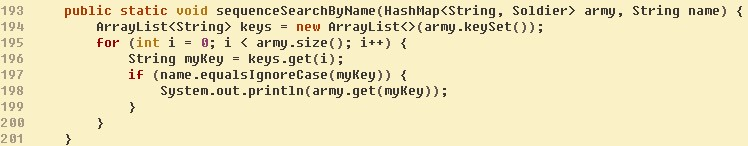
\includegraphics[width=1\textwidth,keepaspectratio]{img/sequence.jpg}
		%\includesvg{img/automata.svg}
		%\label{img:mot2}
		%\caption{Product backlog.}
	\end{figure}
	
	
	\begin{itemize}	
		\item Debido a condiciones de la práctica de laboratorio, se añade un método que hace una búsqueda secuencial. Para lograr ello, se decide guardar las llaves en un ArrayList con la ayuda del método keySet() que está dentro del constructor de ArrayList. Una vez realizado ello, ya podremos hacer uso de la búsqueda secuencial donde se compara la llave (recordemos que la llave es un dato de tipo String) con el String name del parámetro, cuando hayan coincidencias, el valor actual de la variable myKey será usada para poder acceder al valor del HashMap.
	\end{itemize}
	
		\begin{lstlisting}[language=bash,caption={Compilando y probando }][H]
		javac VideoJuego5.java
		java VideoJuego5
		Desea jugar una ronda?(si/no)
		si
		oooooooooooooooo  FASE 1 DE LA CONTIENDA  oooooooooooooooo
		Mostrando estadisticas de cada ejercito
		
		Mostrando soldados por orden de creacion
		DATOS DEL DEL EJERCITO A
		Soldier4X4: Soldier [name=Soldier4X4, lifePoints=1, row=4, column=4]
		Soldier10X4: Soldier [name=Soldier10X4, lifePoints=5, row=10, column=4]
		Soldier2X8: Soldier [name=Soldier2X8, lifePoints=1, row=2, column=8]
		Soldier4X6: Soldier [name=Soldier4X6, lifePoints=3, row=4, column=6]
		Mayor vida en A: Soldier [name=Soldier10X4, lifePoints=5, row=10, column=4]
		El total de vida del ejercito A es: 10
		El promedio de vida del ejercito A es: 2.5
		Mostrando soldados por ranking de poder de A
		Soldier4X4: Soldier [name=Soldier4X4, lifePoints=1, row=4, column=4]
		Soldier2X8: Soldier [name=Soldier2X8, lifePoints=1, row=2, column=8]
		Soldier4X6: Soldier [name=Soldier4X6, lifePoints=3, row=4, column=6]
		Soldier10X4: Soldier [name=Soldier10X4, lifePoints=5, row=10, column=4]
		Ingrese el nombre del Soldier que desea buscar
		soldier4x6
		Se ha encontrado: Soldier [name=Soldier4X6, lifePoints=3, row=4, column=6]
		DATOS DEL EJRCITO B
		Soldier3X1: Soldier [name=Soldier3X1, lifePoints=5, row=3, column=1]
		Soldier2X2: Soldier [name=Soldier2X2, lifePoints=2, row=2, column=2]
		Soldier4X1: Soldier [name=Soldier4X1, lifePoints=3, row=4, column=1]
		Soldier2X6: Soldier [name=Soldier2X6, lifePoints=5, row=2, column=6]
		Soldier1X7: Soldier [name=Soldier1X7, lifePoints=2, row=1, column=7]
		Soldier7X2: Soldier [name=Soldier7X2, lifePoints=5, row=7, column=2]
		Soldier4X3: Soldier [name=Soldier4X3, lifePoints=4, row=4, column=3]
		Soldier10X5: Soldier [name=Soldier10X5, lifePoints=1, row=10, column=5]
		Mayor vida en B: Soldier [name=Soldier7X2, lifePoints=5, row=7, column=2]
		El total de vida del ejercito B es: 27
		El promedio de vida del ejercito B es: 3.375
		Mostrando soldados por ranking de poder de B
		Soldier10X5: Soldier [name=Soldier10X5, lifePoints=1, row=10, column=5]
		Soldier2X2: Soldier [name=Soldier2X2, lifePoints=2, row=2, column=2]
		Soldier1X7: Soldier [name=Soldier1X7, lifePoints=2, row=1, column=7]
		Soldier4X1: Soldier [name=Soldier4X1, lifePoints=3, row=4, column=1]
		Soldier4X3: Soldier [name=Soldier4X3, lifePoints=4, row=4, column=3]
		Soldier3X1: Soldier [name=Soldier3X1, lifePoints=5, row=3, column=1]
		Soldier2X6: Soldier [name=Soldier2X6, lifePoints=5, row=2, column=6]
		Soldier7X2: Soldier [name=Soldier7X2, lifePoints=5, row=7, column=2]
		Ingrese el nombre del Soldier que desea buscar
		soldier1x7
		Soldier [name=Soldier1X7, lifePoints=2, row=1, column=7]
		Desea jugar una ronda?(si/no)
		no
	\end{lstlisting}
	
	
	
	\begin{lstlisting}[language=bash,caption={Commit: a0365cf1eebf124b7cfd8019ec7895186cb90074}][H]
		git add VideoJuego5.java
		git commit -m "Se culmina el metodo de busqueda sencuencial"			
		git push -u origin main
	\end{lstlisting}
	
	



	
	
	\begin{lstlisting}[language=bash,caption={Se modifica el método que imprime el tablero}][H]
		vim VideoJuego5.java
	\end{lstlisting}
	
	\begin{figure}[H]
		\centering
		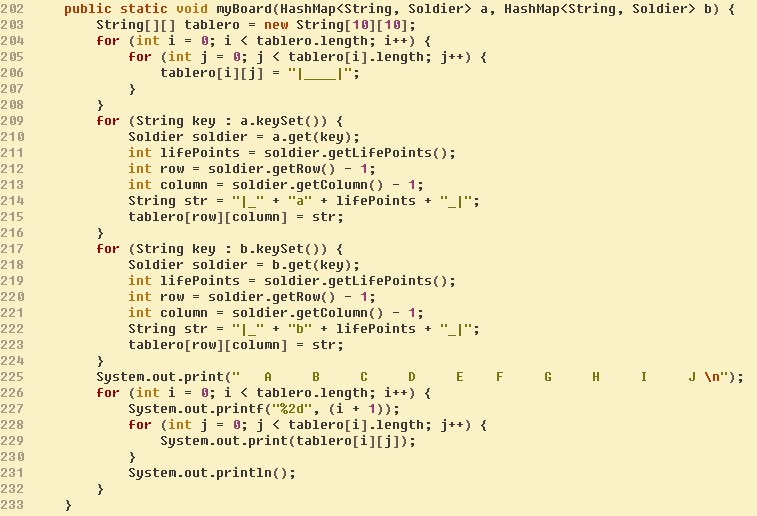
\includegraphics[width=1.1\textwidth,keepaspectratio]{img/myBoard.jpg}
		%\includesvg{img/automata.svg}
		%\label{img:mot2}
		%\caption{Product backlog.}
	\end{figure}
	
	
	\begin{itemize}	
		\item Se hace uso de 4 ciclos for. El primero genera el tablero. El segundo ubica las fichas del ejército A. El tercer for acomoda las fichas del ejército B. El cuarto for que sería anidado muestra el tablero con las fichas incluidas.
	\end{itemize}
	

	
	
	\begin{lstlisting}[language=bash,caption={Compilando y probando el codigo }][H]
		javac VideoJuego5.java
		java VideoJuego5
		Desea jugar una ronda?(si/no)
		si
		oooooooooooooooo  FASE 1 DE LA CONTIENDA  oooooooooooooooo
		Mostrando estadisticas de cada ejercito
		
		Mostrando soldados por orden de creacion
		DATOS DEL DEL EJERCITO A
		Soldier7X3: Soldier [name=Soldier7X3, lifePoints=2, row=7, column=3]
		Soldier4X6: Soldier [name=Soldier4X6, lifePoints=2, row=4, column=6]
		Soldier8X3: Soldier [name=Soldier8X3, lifePoints=3, row=8, column=3]
		Mayor vida en A: Soldier [name=Soldier8X3, lifePoints=3, row=8, column=3]
		El total de vida del ejercito A es: 7
		El promedio de vida del ejercito A es: 2.3333333333333335
		Mostrando soldados por ranking de poder de A
		Soldier7X3: Soldier [name=Soldier7X3, lifePoints=2, row=7, column=3]
		Soldier4X6: Soldier [name=Soldier4X6, lifePoints=2, row=4, column=6]
		Soldier8X3: Soldier [name=Soldier8X3, lifePoints=3, row=8, column=3]
		Ingrese el nombre del Soldier que desea buscar
		soldier5x3
		No se han encontrado coincidencias
		DATOS DEL EJRCITO B
		Soldier3X1: Soldier [name=Soldier3X1, lifePoints=4, row=3, column=1]
		Soldier6X2: Soldier [name=Soldier6X2, lifePoints=5, row=6, column=2]
		Soldier8X1: Soldier [name=Soldier8X1, lifePoints=3, row=8, column=1]
		Soldier1X6: Soldier [name=Soldier1X6, lifePoints=1, row=1, column=6]
		Soldier9X3: Soldier [name=Soldier9X3, lifePoints=4, row=9, column=3]
		Soldier6X6: Soldier [name=Soldier6X6, lifePoints=1, row=6, column=6]
		Soldier7X6: Soldier [name=Soldier7X6, lifePoints=3, row=7, column=6]
		Mayor vida en B: Soldier [name=Soldier6X2, lifePoints=5, row=6, column=2]
		El total de vida del ejercito B es: 21
		El promedio de vida del ejercito B es: 3.0
		Mostrando soldados por ranking de poder de B
		Soldier1X6: Soldier [name=Soldier1X6, lifePoints=1, row=1, column=6]
		Soldier6X6: Soldier [name=Soldier6X6, lifePoints=1, row=6, column=6]
		Soldier8X1: Soldier [name=Soldier8X1, lifePoints=3, row=8, column=1]
		Soldier7X6: Soldier [name=Soldier7X6, lifePoints=3, row=7, column=6]
		Soldier3X1: Soldier [name=Soldier3X1, lifePoints=4, row=3, column=1]
		Soldier9X3: Soldier [name=Soldier9X3, lifePoints=4, row=9, column=3]
		Soldier6X2: Soldier [name=Soldier6X2, lifePoints=5, row=6, column=2]
		Ingrese el nombre del Soldier que desea buscar
		soldier3x1
		Soldier [name=Soldier3X1, lifePoints=4, row=3, column=1]
		
		oooooooooooooooo  FASE 2 DE LA CONTIENDA  oooooooooooooooo
		Mostrando el tablero de juego
		   A      B      C     D      E     F      G      H      I      J
		1 |____||____||____||____||____||_b1_||____||____||____||____|
		2 |____||____||____||____||____||____||____||____||____||____|
		3 |_b4_||____||____||____||____||____||____||____||____||____|
		4 |____||____||____||____||____||_a2_||____||____||____||____|
		5 |____||____||____||____||____||____||____||____||____||____|
		6 |____||_b5_||____||____||____||_b1_||____||____||____||____|
		7 |____||____||_a2_||____||____||_b3_||____||____||____||____|
		8 |_b3_||____||_a3_||____||____||____||____||____||____||____|
		9 |____||____||_b4_||____||____||____||____||____||____||____|
		10|____||____||____||____||____||____||____||____||____||____|
		
		Desea jugar una ronda?(si/no)
		no
	\end{lstlisting}
	
	
	\begin{lstlisting}[language=bash,caption={Commit: 6a85e033318ba91b893414da2a57263477c07c71}][H]
		git add VideoJuego5.java
		git commit -m "Metodo myBoard ha sido terminado"			
		git push -u origin main
	\end{lstlisting}
	
		
	\subsection{Métodos que ya estaban y que no fueron modificados}
	
	\begin{figure}[H]
		\centering
		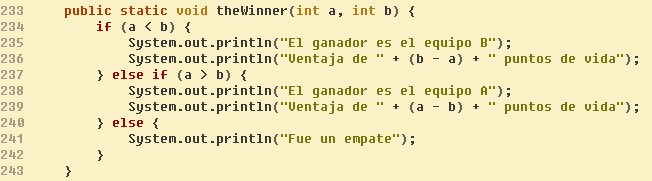
\includegraphics[width=1\textwidth,keepaspectratio]{img/theWinner.jpg}
		%\includesvg{img/automata.svg}
		%\label{img:mot2}
		%\caption{Product backlog.}
	\end{figure}
	
	
	\begin{itemize}	
		\item theWinner: Este método trabajado en la actividad pasada determina al ganador o si hubo empate.
	\end{itemize}
	
	\begin{figure}[H]
		\centering
		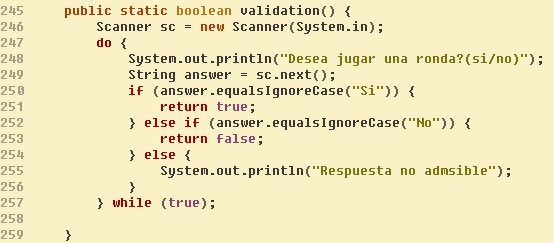
\includegraphics[width=1\textwidth,keepaspectratio]{img/validation.jpg}
		%\includesvg{img/automata.svg}
		%\label{img:mot2}
		%\caption{Product backlog.}
	\end{figure}
	
	
	\begin{itemize}	
		\item validation: Este método hace psoible que el programa sea iterativo.
	\end{itemize}
	
		\begin{lstlisting}[language=bash,caption={Compilando y probando el codigo en su versión final }][H]
		javac VideoJuego5.java
		java VideoJuego5
		Desea jugar una ronda?(si/no)
		si
		oooooooooooooooo  FASE 1 DE LA CONTIENDA  oooooooooooooooo
		Mostrando estadisticas de cada ejercito
		
		Mostrando soldados por orden de creacion
		DATOS DEL DEL EJERCITO A
		Soldier9X3: Soldier [name=Soldier9X3, lifePoints=4, row=9, column=3]
		Soldier4X9: Soldier [name=Soldier4X9, lifePoints=4, row=4, column=9]
		Soldier2X9: Soldier [name=Soldier2X9, lifePoints=5, row=2, column=9]
		Soldier4X7: Soldier [name=Soldier4X7, lifePoints=5, row=4, column=7]
		Soldier7X7: Soldier [name=Soldier7X7, lifePoints=1, row=7, column=7]
		Soldier8X7: Soldier [name=Soldier8X7, lifePoints=2, row=8, column=7]
		Mayor vida en A: Soldier [name=Soldier4X7, lifePoints=5, row=4, column=7]
		El total de vida del ejercito A es: 21
		El promedio de vida del ejercito A es: 3.5
		Mostrando soldados por ranking de poder de A
		Soldier7X7: Soldier [name=Soldier7X7, lifePoints=1, row=7, column=7]
		Soldier8X7: Soldier [name=Soldier8X7, lifePoints=2, row=8, column=7]
		Soldier9X3: Soldier [name=Soldier9X3, lifePoints=4, row=9, column=3]
		Soldier4X9: Soldier [name=Soldier4X9, lifePoints=4, row=4, column=9]
		Soldier2X9: Soldier [name=Soldier2X9, lifePoints=5, row=2, column=9]
		Soldier4X7: Soldier [name=Soldier4X7, lifePoints=5, row=4, column=7]
		Ingrese el nombre del Soldier que desea buscar
		soldier9x3
		Se ha encontrado: Soldier [name=Soldier9X3, lifePoints=4, row=9, column=3]
		DATOS DEL EJRCITO B
		Soldier8X3: Soldier [name=Soldier8X3, lifePoints=2, row=8, column=3]
		Soldier9X8: Soldier [name=Soldier9X8, lifePoints=5, row=9, column=8]
		Soldier2X10: Soldier [name=Soldier2X10, lifePoints=5, row=2, column=10]
		Mayor vida en B: Soldier [name=Soldier2X10, lifePoints=5, row=2, column=10]
		El total de vida del ejercito B es: 12
		El promedio de vida del ejercito B es: 4.0
		Mostrando soldados por ranking de poder de B
		Soldier8X3: Soldier [name=Soldier8X3, lifePoints=2, row=8, column=3]
		Soldier9X8: Soldier [name=Soldier9X8, lifePoints=5, row=9, column=8]
		Soldier2X10: Soldier [name=Soldier2X10, lifePoints=5, row=2, column=10]
		Ingrese el nombre del Soldier que desea buscar
		soldier8x3
		Soldier [name=Soldier8X3, lifePoints=2, row=8, column=3]
		
		oooooooooooooooo  FASE 2 DE LA CONTIENDA  oooooooooooooooo
		Mostrando el tablero de juego
		   A      B      C     D      E     F      G      H      I     J
		1 |____||____||____||____||____||____||____||____||____||____|
		2 |____||____||____||____||____||____||____||____||_a5_||_b5_|
		3 |____||____||____||____||____||____||____||____||____||____|
		4 |____||____||____||____||____||____||_a5_||____||_a4_||____|
		5 |____||____||____||____||____||____||____||____||____||____|
		6 |____||____||____||____||____||____||____||____||____||____|
		7 |____||____||____||____||____||____||_a1_||____||____||____|
		8 |____||____||_b2_||____||____||____||_a2_||____||____||____|
		9 |____||____||_a4_||____||____||____||____||_b5_||____||____|
		10|____||____||____||____||____||____||____||____||____||____|
		
		+++++++++++++++++   FASE 3 DE LA CONTIENDA  +++++++++++++++++
		El ganador se determina en base a los puntos de vida total
		Enfrentamiento
		El ganador es el equipo A
		Ventaja de 9 puntos de vida
		Desea jugar una ronda?(si/no)
		no
	\end{lstlisting}
	
	
	\begin{lstlisting}[language=bash,caption={Commit: 4343ad638f404dafc97349ff35c8808998ea0f1b}][H]
		git add VideoJuego5.java
		git commit -m "En el main se prepara lo necesario para determinar al ganador"			
		git push -u origin main
	\end{lstlisting}
	
	\subsection{Diagrama UML y el main}
	
	\begin{figure}[H]
		\centering
		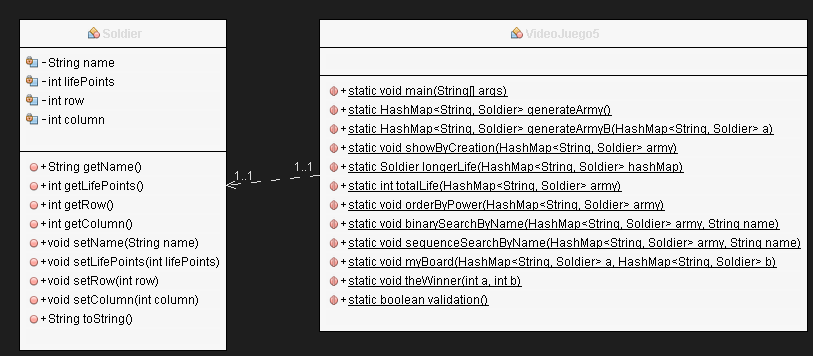
\includegraphics[width=1\textwidth,keepaspectratio]{img/uml.png}
		%\includesvg{img/automata.svg}
		%\label{img:mot2}
		%\caption{Product backlog.}
	\end{figure}
	
	\begin{figure}[H]
		\centering
		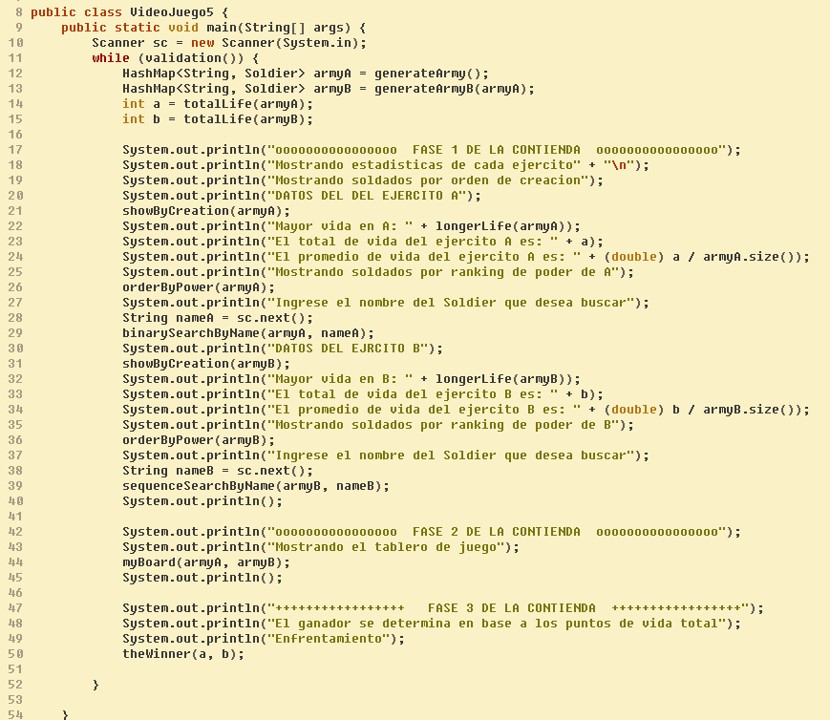
\includegraphics[width=1\textwidth,keepaspectratio]{img/main.jpg}
		%\includesvg{img/automata.svg}
		%\label{img:mot2}
		%\caption{Product backlog.}
	\end{figure}
	
	\subsection{Estructura de laboratorio 08}
	\begin{itemize}	
		\item El contenido que se entrega en este laboratorio es el siguiente:
	\end{itemize}
	
	\begin{lstlisting}[style=ascii-tree]
		lab08
		|   
		|	  Soldier.java
		|    VideoJuego5.java
		|
		 ─ ─latex
			  |  	 programacion_lab08_rescobedoq_v1.0.pdf
			  |    programacion_lab08_rescobedoq_v1.0.tex
			  |
			   ─ ─ img
							average.jpg
							binary.jpg
							binarySearchByName.jpg
							burbuja.jpg
							classSoldier.jpg
							generateArmy.jpg
							generateArmyB.jpg
							insertion.jpg
							logo_abet.png
							logo_episunsa.png
							logo_unsa.jpg
							longerLife.jpg
							main.jpg
							myBoard.jpg
							orderByPower.jpg
							sequence.jpg
							showByCreation.jpg
							theWinner.jpg
							totalLife.jpg
							uml.png
							validation.jpg
			
	\end{lstlisting}    
	
	\section{\textcolor{red}{Rúbricas}}
	
	\subsection{\textcolor{red}{Entregable Informe}}
	\begin{table}[H]
		\caption{Tipo de Informe}
		\setlength{\tabcolsep}{0.5em} % for the horizontal padding
		{\renewcommand{\arraystretch}{1.5}% for the vertical padding
			\begin{tabular}{|p{3cm}|p{12cm}|}
				\hline
				\multicolumn{2}{|c|}{\textbf{\textcolor{red}{Informe}}}  \\
				\hline 
				\textbf{\textcolor{red}{Latex}} & \textcolor{blue}{El informe está en formato PDF desde Latex,  con un formato limpio (buena presentación) y facil de leer.}   \\ 
				\hline 
				
				
			\end{tabular}
		}
	\end{table}
	
	\clearpage
	
	\subsection{\textcolor{red}{Rúbrica para el contenido del Informe y demostración}}
	\begin{itemize}			
		\item El alumno debe marcar o dejar en blanco en celdas de la columna \textbf{Checklist} si cumplio con el ítem correspondiente.
		\item Si un alumno supera la fecha de entrega,  su calificación será sobre la nota mínima aprobada, siempre y cuando cumpla con todos lo items.
		\item El alumno debe autocalificarse en la columna \textbf{Estudiante} de acuerdo a la siguiente tabla:
		
		\begin{table}[ht]
			\caption{Niveles de desempeño}
			\begin{center}
				\begin{tabular}{ccccc}
					\hline
					& \multicolumn{4}{c}{Nivel}\\
					\cline{1-5}
					\textbf{Puntos} & Insatisfactorio 25\%& En Proceso 50\% & Satisfactorio 75\% & Sobresaliente 100\%\\
					\textbf{2.0}&0.5&1.0&1.5&2.0\\
					\textbf{4.0}&1.0&2.0&3.0&4.0\\
					\hline
				\end{tabular}
			\end{center}
		\end{table}	
		
	\end{itemize}
	
	\begin{table}[H]
		\caption{Rúbrica para contenido del Informe y demostración}
		\setlength{\tabcolsep}{0.5em} % for the horizontal padding
		{\renewcommand{\arraystretch}{1.5}% for the vertical padding
			%\begin{center}
			\begin{tabular}{|p{2.7cm}|p{7cm}|x{1.3cm}|p{1.2cm}|p{1.5cm}|p{1.1cm}|}
				\hline
				\multicolumn{2}{|c|}{Contenido y demostración} & Puntos & Checklist & Estudiante & Profesor\\
				\hline
				\textbf{1. GitHub} & Hay enlace URL activo del directorio para el  laboratorio hacia su repositorio GitHub con código fuente terminado y fácil de revisar. &2 &X &2 & \\ 
				\hline
				\textbf{2. Commits} &  Hay capturas de pantalla de los commits más importantes con sus explicaciones detalladas. (El profesor puede preguntar para refrendar calificación). &4 &X &4 & \\ 
				\hline 
				\textbf{3. Código fuente} &  Hay porciones de código fuente importantes con numeración y explicaciones detalladas de sus funciones. &2 &X &2 & \\ 
				\hline 
				\textbf{4. Ejecución} & Se incluyen ejecuciones/pruebas del código fuente  explicadas gradualmente. &2 &X &2 & \\ 
				\hline			
				\textbf{5. Pregunta} & Se responde con completitud a la pregunta formulada en la tarea.  (El profesor puede preguntar para refrendar calificación).  &2 &X &2 & \\ 
				\hline	
				\textbf{6. Fechas} & Las fechas de modificación del código fuente estan dentro de los plazos de fecha de entrega establecidos. &2 &X &2 & \\ 
				\hline 
				\textbf{7. Ortografía} & El documento no muestra errores ortográficos. &2 &X &1 & \\ 
				\hline 
				\textbf{8. Madurez} & El Informe muestra de manera general una evolución de la madurez del código fuente,  explicaciones puntuales pero precisas y un acabado impecable.   (El profesor puede preguntar para refrendar calificación).  &4 &X &3 & \\ 
				\hline
				\multicolumn{2}{|c|}{\textbf{Total}} &20 & &18 & \\ 
				\hline
			\end{tabular}
			%\end{center}
			%\label{tab:multicol}
		}
	\end{table}
	
	\clearpage
	
	\section{Referencias}
	\begin{itemize}			
		\item \url{https://www.geeksforgeeks.org/binary-search/}
		\item \url{https://www.geeksforgeeks.org/insertion-sort/}
	\end{itemize}	
	
	%\clearpage
	%\bibliographystyle{apalike}
	%\bibliographystyle{IEEEtranN}
	%\bibliography{bibliography}
	
\end{document}